\chapter{Social Routing Service}

The Social Routing Service (SRS) is comprised of three major components, 
A Database Management System (DBMS) to store user related information, a server to process data and an API to expose it's functionality.
This logic is represented in the figure \ref{fig:socialroutingservice}. Beyond the mentioned
components it also uses the external API Google Sign In to aid with the user authentication process.

\begin{figure}[ht]            
    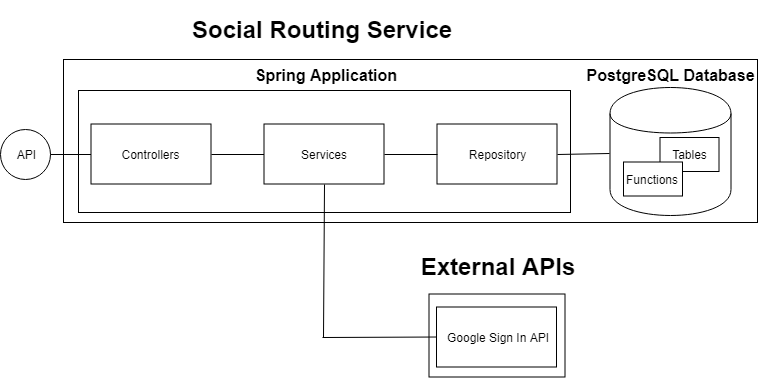
\includegraphics[width=\textwidth]{images/project-structure/service-structure2.PNG}
    \caption{Social Routing Service architecture.}
    \label{fig:socialroutingservice}
\end{figure}  

The components, although separated, must communicate with each other in order for the SRS
to function properly. The API is exposed by the server using the HTTP protocol. The 
communication with external APIs made by the server is done through the HTTPS\cite{https} 
protocol.

The communication with the DBMS is made using JDBI\cite{jdbidocs}, a library built on top
of the JDBC\cite{jdbcdocs} driver. The main idea when building the communication with the DBMS
was to guarantee that a single request made to the service would use a single connection 
to the DBMS. For that reason, the connection is both created and closed in the controller
element of the system. This way it allows that the DBMS connection is used multiple times
by the same request if required.
\newpage

\section*{Database Management System}
The DBMS chosen was PostgreSQL\cite{postgresql}, using the hybrid functionality 
of storing valid JSON\cite{postgresqljson} directly in a table field. The decision of choosing JSON as a type to 
store data comes with the need of storing large sets of coordinates belonging to a single entity and this 
allows us to make faster and easier calculations of times and distances between routes and points rather than if a 
point was it's own database entity. 
The main concept of the project is the creation of routes in a map and their retrieval according to certain parameters.
To consider distance between a user and a route a possible search parameter, the PostGIS\cite{postgis} 
PostgreSQL extension was used as it allows both cartesian and geodesic distance calculations.

    \subsection*{Conceptual Model}
    The database entity diagram is shown in figure \ref{fig:erdiagram}.

    \begin{figure}[ht]            
        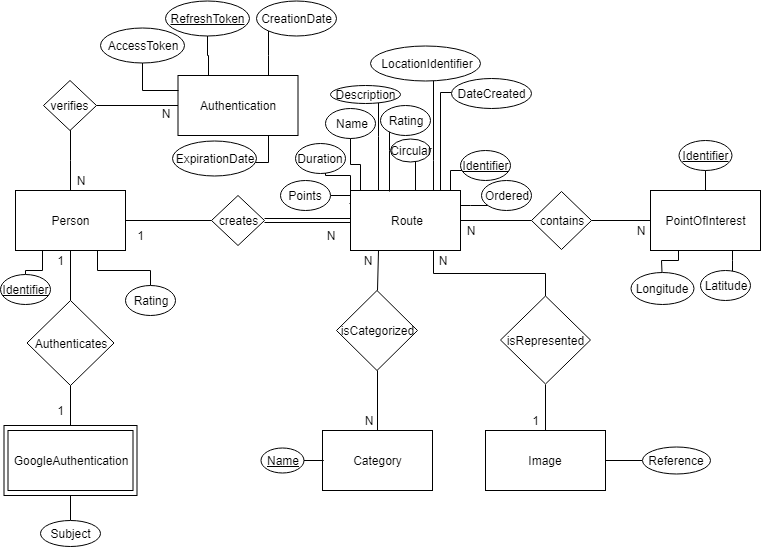
\includegraphics[width=\textwidth]{images/project-structure/dbms-structure.PNG}
        \caption{Entity Relationship Diagram.}
        \label{fig:erdiagram}
    \end{figure}   

        \subsubsection*{Person}
        The entity Person represents a single user in the database. To allow new forms of authentication to be introduced at a later time,
        the Google Authentication table is separated from the Authentication one. A user can have multiple entries
        on the Authentication table to enable multiple device registration, but only a single Google Authentication 
        entry as the google account is unique.

        \subsubsection*{Route}
        Entity that stores every information required to hold a Route. Special consideration was taken into the making
        of this entity as a Route must have large sets of coordinates, representing the path that it undergoes. The 
        use of JSON as a table field Points provided more customization and a more efficient way to make calculations 
        of distances between routes and points. 

        \subsubsection*{GoogleAuthentication}
        Google Authentication is the entity that stores the user unique identifier in the Google platform, the subject, as such,
        a user can only have one entry in the GoogleAuthentication table.
        In the future there will be multiple tables with different forms of authentication, hence the name GoogleAuthentication 
        of the entity. It provides scalability to further augment the authentication process, which can be done
        with a new table FacebookAuthentication for example.

        \subsubsection*{Authentication}
        This entity is used to store authentication metadata regarding each database user. The tokens have an expiration time,
        and because of it their creation date is required as well as their expiration date.

        \subsubsection*{Category}
        The category entity defines a route in a broader sense. It is used to filter the amount of routes being 
        searched by a user. It can be one of the several: Sea, Sports, Cultural, amongst others.
        Each route must be assigned at least one category.

        \subsubsection*{PointOfInterest}
        A route might contain geographic points of interest along its path, this is the entity that represents them. 

        \subsubsection*{Image}
        When a route is created it must be associated with a cover image. 

    \subsection*{Physical Model}
    The physical model can be seen in a detailed form in the DBMS documentation.\cite{servicedbms}

    \subsection*{Search Route}
    The SRS allows that a client searches routes that are nearby to a set of geographic coordinates (latitude and longitude). 
    This functionality could be implemented in either the server or the DBMS, but with the PostGIS capabilities already mentioned, the later was chosen.
    
    The search by proximity algorithm is built on two phases, the initial filtering by data received as parameter, to reduce the amount of 
    calculations required, and the calculations on the resulting set of routes to check if they belong to a user area or not.
    
    More specifically, when searching for routes close to a user's coordinates, the initial parameters must be the lower bound radius
    and the upper bound radius. These parameters build a circumference around the user's coordinates that goes from the lower radius to the 
    upper one. With these parameters, if no routes are found in the specified radius, the radius can be increased or decreased in repeated
    searches without incurring in the overhead of filtering the already discarded routes. 

    The following example illustrates the data required to make such search:
    A user has the coordinates 38.755833, -9.116667 and is searching for short routes, that are sports related.
    With this data, first the city where the coordinates belong is found. After that, a query is made to the database
    to find which routes in the given coordinates city are short and sports related. This is the first phase of filtering.
    The second phase is to filter the retrieved routes by distance to the original coordinates. If they are inside the 
    given radius, they are selected, if not, discarded.

    To be able to calculate if a route belongs to a user given area, the user coordinates are transformed into a Geographic Object\cite{geographicobject},
    then, each of the already filtered and retrieved routes is checked for distance to that geographic object. To be noted that the construction of a geographic
    object is necessary because the calculations being made are not made on the cartesian plane but on the spatial one. They must be made considering a spherical 
    object to provide accurate results (in case a long distance between route points exists). Of course each route contains every geographic point in its field points,
    which is of type JSON. Of of each of the routes the points must be extracted and converted into the same Geographic Object type. From here, using the built in function
    of the PostGIS extension STDistance \cite{stdistance}, the distance between points is retrieved, if it's contained in the initially 
    chosen radius, it's selected, otherwise it is not.

\section*{Social Routing API}    
    \subsection*{Schema}
        The Social Routing API uses the HTTP protocol as a medium to 
        communicate and all the data sent or received must be in the JSON format.
        The base endpoint of the API is : http://api.sr.\par
        Data obtained from the API is either a single resource or a collection of resources. For example, a request
        made to retrieve a route will have as a response a single resource which will contain the representation of that
        route. If a request is made to obtain routes by location then the response will be a collection of resources containing
        the several route representations. This single and collection terms when associated with a
        resource were decisive in the choice of how much data would be returned in either of them. A request for a collection
        doesn't require detailed information about each element of the collection, it needs to provide general information and
        a form for the API user to retrieve detailed information about a specific collection element.
        With this idea in mind the resource representations were divided into two types, a detailed representation for when a user
        requests a single resource and summary representation for each element inside a requested collection, containing only the 
        information about that element that is necessary.
        Examples of both a detailed and summary representation can be found in the Schema Documentation \cite{schemadocs}.    
    
        \newpage
    
    \subsection*{Authentication}
    The API's authentication is made with the support of the Google Sign-In API. 
    The authentication is done in two phases. The first phase is the registration of a new user. 
    On this phase a POST \cite{httppostdocs} request must be made to the endpoint: http://api.sr/sign-in/google, 
    with the Google Sign-In token in the body of the request:
    \begin{lstlisting}
    {
      token : "Google Sign-In token"
    }
     \end{lstlisting}
    The token is provided by the Google Sign-In API and when it's received in the Service's API, 
    it's authenticity is verified using the Google Sign-in-API utilities. After the validity of the token is verified 
    the subject field is extracted from it to identify the user performing the registration and stored by the service. 
    Then an API token is generated from a time based unique identifier generator, provided by the Log4J library \cite{log4j},
    and associated to the previously received subject. Before being stored the token is hashed to increase security. 
    The response to the request will contain the generated token in it's original form so the user haves the required information 
    to make authenticated requests from there on.\par

    The second phase of the authentication process is made in any request that follows user registration. The API user must 
    send a request containing the previously received token in the Authorization HTTP header. When any request is received 
    the headers are retrieved, and checked against the service's database. In this check, the received token is hashed and 
    compared to the hashed version on the database, if no token with that hash is present then the authentication fails 
    and the user receives an error response.

    \newpage
    \subsection*{Supported HTTP Methods}
        Due to the nature of the HTTP protocol, the API supports four different HTTP request methods \cite{apihttpverbsdocs}: GET, POST, PUT and DELETE.
        
        \subsubsection*{GET}
        This method is used to retrieve resources from the API. The request: 
        \begin{verbatim}
            GET http://api.sr/persons/1 
        \end{verbatim}
        \vspace{-\baselineskip}
        retrieves a resource representing a person resource with the identifier 1. 
        The response to this request would be:
        \begin{lstlisting}
        {
          "identifier": 1,
          "rating": 4,
          "routesUrl": "http://api.sr/persons/1/routes"
        }
        \end{lstlisting}

        \subsubsection*{POST}
        The POST HTTP method is used to create resources. It requires that the Content-Type\cite{contenttype}HTTP header is 
        defined and with the value application/json\cite{applicationjson}. An example of a post request can be found in the 
        API POST\cite{apipostdocs} documentation. A response to a POST request has an empty body and returns the 
        location of the created resource in it's Location header. If successful the status code of a POST request response is 201.  
            
        \subsubsection*{PUT}
        The PUT method is used to replace or update a resource or a collection of resources. Like the post request it requires 
        that the request contains the HTTP header Content-Type defined with application/json.
        The following request replaces the currently existing resource route with identifier 1 with the one sent in 
        the body of the request. A successful response has the 200 OK status and an empty body. An example of a put 
        request can be found in the API PUT\cite{apiputdocs} documentation.

        \subsubsection*{DELETE}
        DELETE, as the name implies is utilized to delete a resource. The request: 
        \begin{verbatim}
            DELETE http://api.sr/routes/1
        \end{verbatim}
        \vspace{-\baselineskip} 
        deletes the route with 1 as identifier. A successful response will have the 200 OK status and an empty body.
    
    \subsection*{Pagination}
    Requests that return a collection of resources will be paginated to a default value of 5 resources within the collection. 
    A specific page can be requested with the query parameter page. 
    The request:  
    \begin{verbatim}
        GET http://api.sr/persons/1/routes?page=1
    \end{verbatim}
    \vspace{-\baselineskip}
     returns the first five routes that a person with identifier 1 created.
    To obtain the next 5 one would simply change de value of page to 2.

    \subsection*{Errors}
    The error responses follow the RFC standard of type problem+json\cite{jsonproblemonlinedocs}. An error response example:
    
    \begin{lstlisting}
    {
      "type": "Social-Routing-API#unsupported-media-type\cite{unsupportedmedia}",
      "title": "The requested type is not supported.",
      "status": "415",
      "detail": "The xml format is not supported."
    }
    \end{lstlisting}

    \subsection*{Hypermedia}
    Some resources have links to other resources. Either to a parent resource or to a detailed representation of a 
    resource within a collection. For example, a user resource haves a link to their created routes, which 
    holds a collection of routes. That same collection haves a link to the profile of the person who created 
    the routes.
    \newpage

\section*{Server} 
The server uses Kotlin as a programming language and the Spring framework\cite{springwebsite}. 
It's role within the system is data receival, data processing, 
and to respond accordingly. It is divided in three major layers, each with it's role in the Social Routing Service's system. 
They are the Controllers, the Services and the Repository.

The Controllers are responsible for handling the reception of an HTTP request to the service and are mapped to
it's endpoints. Upon receiving a request they will use the available services to perform desired operations either
over a set of received data or to generate the requested data.

The Services are responsible for processing data and communicating the the Repository layer.

The Repository layer is the only layer with direct access to the database and as such is responsible for communicating
with it. The communication is made through the use of JDBI\cite{jdbidocs}, a library built on top of the driver JDBC\cite{jdbcdocs}. This allows
less verbose code while maintaining control over SQL queries. 

Besides these three major layers the server contains other important components, the Interceptor\cite{springinterceptor} and the Exception Handler\cite{springexception}.
There are three different implementations of the Interceptor component.

The Authentication Interceptor is responsible for user authentication before the request reaches a controller. The goal of this
implementation is to avoid server overhead, resolving the authentication before the request is processed allows for a fast response
if the user is incorrectly authenticated instead of continuing with the unnecessary processing of data.

The Logging Interceptor is used both before and after the request is processed to provide information 
regarding each request for debugging purposes.

The Media Type Interceptor is used, like the Authentication Interceptor, to avoid overhead, since if a post request is made
with wrong Content-Type headers or no headers at all then the service does not support that request and can respond with an 
error immediately.

The Exception Handler is the component responsible for the handling of exceptions of the system. In the Spring framework there 
are several ways to handle exceptions, but the choice to make is to either handle the exceptions locally or globally. The 
handler implementation groups all the exceptions thrown by the system in a single class and produces their respective error 
messages. It allows for an easier work flow when treating exceptions. The global handling was chosen because most of the 
exceptions happen in more than one endpoint and would produce a lot of repeated code if handled locally.      
\newpage
As an example, the flow of a correct HTTP POST request to the routes resource that arrives on the server is the following:
    \begin{itemize}
        \item The request is intercepted by the Logging Interceptor and logs the request information.
        \item It is then intercepted by the Media Type Interceptor, that checks if the request data format 
        received is supported by the service.
        \item The Authentication Interceptor checks the user credentials to see if the user can indeed access the service.
        \item The endpoint is reached in it's mapped Controller, which receives the Route information and that it 
        maps to the correct object. In this case the Route Controller which will then call a service responsible 
        for processing the request data.
        \item The service, in this case Route Service, will process the data and map it  to the correct data type 
        and make a request to the repository to store the received data.
        \item The repository communicates with the database, to which it sends the data in a database accepted format.
        \item The database stores the data and returns the identifier of the newly created Route.
        \item The repository receives the identifier and passes it through to the Route Service.
        \item The Service passes the received information to the Route Controller.
        \item The Route Controller builds the newly created route resource URI with the received Route identifier 
        and maps it to the header Location of the response and returns.
    \end{itemize}
    \newpage
